\documentclass[journal]{IEEEtran}

% ---------------------------------------------------------------- packages
\usepackage[T1]{fontenc}
\usepackage{amsmath,amssymb}
\usepackage{graphicx}
\usepackage{booktabs}
\usepackage{microtype}
\usepackage{siunitx}
\sisetup{range-phrase=--, range-units=single, separate-uncertainty=true, group-digits=integer}
\usepackage[hidelinks]{hyperref}
\usepackage{cite}

% ---------------------------------------------------------------- todo notes
% Set to true to hide every \todo{} for a clean version.
\newif\iffinal
\finalfalse
\iffinal
  \newcommand{\todo}[1]{}
\else
  \usepackage[colorinlistoftodos,textsize=scriptsize]{todonotes}
  \setuptodonotes{inline,color=yellow!40}
\fi

\graphicspath{{figures/}}

% ---------------------------------------------------------------- notation
\newcommand{\neff}{n_\mathrm{eff}}
\newcommand{\ngr}{n_\mathrm{g}}
\newcommand{\nsi}{n_\mathrm{Si}}
\newcommand{\nox}{n_\mathrm{ox}}
\newcommand{\sth}{\sigma_\theta}

\begin{document}

\title{Identifiability of the Waveguide Sidewall Angle in Silicon Photonic Test Structures}

\author{\todo{author names: Unmol Sharma and David [co-author surname]}Unmol~Sharma and David~[LAST NAME]%
\thanks{\todo{manuscript dates}Manuscript received [date]; revised [date].}%
\thanks{\todo{affiliations and e-mails of both authors}U.~Sharma is with Vanderbilt University, Nashville, TN, USA (e-mail: [e-mail]).
D.~[LAST NAME] is with the SOL Lab, Vanderbilt University, Nashville, TN, USA (e-mail: [e-mail]).}%
\thanks{\todo{corresponding author}}}

\maketitle

\begin{abstract}
Ring and interferometer test structures monitor the width and thickness of silicon waveguides across a wafer, but
none reports the sidewall angle, and a tilt that a width fit absorbs mispredicts rib devices by hundreds of
picometres. We ask which test structures make the angle identifiable. For an oxide-clad strip the mode is
mirror-symmetric, so to first order a wall tilt is exactly a width change, and no set of strips can
separate the two. A partially etched rib breaks the symmetry, but a rib from a
separate etch brings its own depth and angle, and one rib width then leaves the strip angle unidentifiable even when
the depth is known. Two widths of the same rib restore identifiability. With rings on several strip widths and two
rib widths, the Cram\'er--Rao bound on the strip angle is \qty{0.39}{\degree} at a \qty{1}{pm} resonance-wavelength
precision, with the etch parameters and material indices unknown. The bound assumes that all structures share one
set of process parameters. It doubles once their widths differ by \qty{0.039}{nm}, so a working test structure must
co-locate its members or measure their differences. Results come from finite-element mode solutions, Fisher
information and nonlinear fits to simulated data.
\end{abstract}

\begin{IEEEkeywords}
Silicon photonics, sidewall angle, test structures, identifiability, Fisher information, Cram\'er--Rao bound, ring
resonators, process monitoring.
\end{IEEEkeywords}

\section{Introduction}
\label{sec:intro}

Suppose the fully etched strips of a silicon photonic process come out with walls tilted by \qty{1}{\degree} and the
monitor rings are fitted with vertical walls. In our simulations the fit absorbs the tilt as a width change of
\qty{-3.8403}{nm}, and a ring made of a \qty{500}{nm} rib on a \qty{90}{nm} slab, predicted from that width, lands
\qty{710.8}{pm} away from where it actually resonates. For comparison, Zortman \textit{et~al.}\ held microdisk resonances to within
\qty{105}{GHz} inside a die~\cite{zortman2010}, which is \qty{841.5}{pm} at \qty{1550}{nm}. Post-fabrication trimming
sets rings to within \qty{\pm 32}{pm} of target~\cite{jayatilleka2021}. An unmonitored degree of sidewall angle is therefore
an error of the same size as the within-die spread that process monitoring is meant to explain. It arises because a
rib's resonance responds to wall tilt differently from a strip's, so a width that matches the strips is wrong for
the ribs.

The optical test structures that foundries and designers use measure the effective and group indices of a few
waveguides and convert them into a width and a thickness~\cite{xing2018,zortman2010,lu2017}. The sidewall angle
enters that conversion as a fixed input. Xing \textit{et~al.}\ took the \qty{85}{\degree} of the foundry handbook and
noted that the error from the unknown wall shape is very hard to compensate, so that some extracted parameters are
only relative~\cite{xing2018}. In this paper we show that, for oxide-clad strips, the omission is forced by the
structures. To first order the angle cannot be separated from the width for any number of strips, widths,
polarizations or readouts. We then work out which additional structures make the angle identifiable, how much prior
process knowledge they need, and what precision they reach under a measurement model built from published ring
metrology~\cite{janz2023}. We then ask what the practical limit is. The result depends on the assumption, common to all multi-device
extraction, that the structures share one set of process parameters, and most of the paper's practical conclusions concern what
happens when they do not.

This is a computational study of test-structure design and identifiability. Every number comes from full-vector
finite-element mode solutions, Fisher information or nonlinear fits of simulated data, and no device was fabricated.
The strip result is first-order and holds for the symmetric oxide-clad cross-section under the measurement model of
Section~\ref{sec:theory}.

\subsection{Related work}

\textit{Optical extraction of waveguide geometry.} Xing \textit{et~al.}\ fitted the effective and group indices of a
low-order and a high-order MZI, mapped them to linewidth and thickness with a third-order polynomial, and reached
total errors of \qty{0.37}{nm} and \qty{0.26}{nm} on 44 sites of an MPW die; they also showed how the index range
must be bounded for the inversion to pick the right interference order~\cite{xing2018}. Later work extracted the same two dimensions
from a single high-order MZI~\cite{liu2025}, from racetrack resonators feeding a layout-aware variability
model~\cite{lu2017}, from ring biosensors read in TE and TM~\cite{atsumi2012}, and from microdisks read in both
polarizations~\cite{zortman2010}. MZI sets have mapped the effective index and its thermo-optic coefficient across
wafers~\cite{dwivedi2015}. For silicon nitride, unbalanced MZIs determined thickness, width offset and both material
indices across a \qty{300}{mm} wafer~\cite{butt2024}. Rib waveguides have been characterized with two racetracks of
different perimeter, with a cross-section estimate checked against STEM~\cite{zhang2024}. A recent patent
application determines the geometry from many resonances of one ring. In its background, it states that methods
using several devices must assume that the devices share the same width and thickness variations, and that this
condition ``is recognized as often not satisfied''~\cite{nrc2026}. None of these works extracts the sidewall angle.

\textit{Fabrication variability.} Width and thickness vary systematically with layout and position. Hierarchical
models separate layout-dependent from random contributions and tie die-scale linewidth variation to pattern
density~\cite{xing2023}, and the resonance mismatch between identical rings grows linearly with their
separation~\cite{chrostowski2014}. CMOS-line fabrication has reached linewidth control better than \qty{0.6}{nm}
within a chip and \qty{2}{nm} chip-to-chip~\cite{selvaraja2010}. Wafer-scale resonator statistics~\cite{robinson2025,mdpi2025,aim2023}
and variability-aware design flows~\cite{bogaerts2018} show why such numbers matter for yield. Ring basics,
including the relation between resonance, free spectral range and group index, are reviewed
in~\cite{bogaerts2012,chrostowski2015}.

\textit{Sidewall angle and physical metrology.} Angled sidewalls break the vertical symmetry of a waveguide and cause
TM-to-TE hybridization and conversion in tapers~\cite{dai2015,mdpi2021}, the mechanism behind some polarization
rotators~\cite{dai2011}. Sidewall roughness causes backscattering and polarization rotation~\cite{morichetti2010}
and sets the loss floor of high-Q rings~\cite{biberman2012}. Dimensional metrology measures the profile directly.
Cross-sectional TEM is destructive and AFM and SEM are local~\cite{orji2018}. 3D-AFM resolves sidewalls of vertical and
undercut structures with die-level reproducibility better than \qty{2}{\percent}~\cite{yoo2022}. Scatterometry is
fast but model-based, and its inverse problem can have correlated parameters and non-unique
solutions~\cite{raymond2005,orji2018}.

\textit{Experiment design and identifiability.} The Cram\'er--Rao lower bound (CRLB) and Fisher information are the
standard tools for asking how well a parameter can be estimated from a measurement~\cite{kay1993}, and optimal
experiment design chooses measurements to improve them~\cite{pukelsheim2006}. A parameter is structurally
unidentifiable when the model output cannot distinguish it from others for any data~\cite{bellman1970}, and
practically unidentifiable when finite, noisy data leave it unbounded~\cite{raue2009}. In dimensional metrology the
Fisher matrix has been used to choose the wavelength and angles of EUV scatterometry so as to break parameter
correlations~\cite{klein2025}, and simulation studies have mapped the sensitivity limits of optical CD
metrology~\cite{silver2007}. Offset and model errors in inverse scatterometry have been propagated to the fitted
profile~\cite{alassaad2007} and estimated jointly with it~\cite{henn2012}. In optics more broadly, Fisher
information has guided the design of maximally informative illumination~\cite{bouchet2021}.

\subsection{Contribution}

Previous optical extraction leaves the sidewall angle out. Previous identifiability-driven metrology design chooses how
to measure one fixed structure. Here we choose which waveguides to measure, and we show that the choice decides
whether the angle is identifiable at all. Specifically:
\begin{itemize}
\item We show, to first order and confirm with mode solutions, that oxide-clad strips are exactly blind to the
sidewall angle, with the angle/width ratio $R=(y_c-y_\mathrm{pivot})/(h/2)$ set by the centroid of the
wall-perturbation weight.
\item We give a counting argument, confirmed by the Fisher matrix and by nonlinear fits, that one rib from a separate
etch leaves the strip angle unidentifiable, and that a known etch depth does not change this.
\item We find that two widths of the same rib restore identifiability. A ring-only set of five strips and two ribs
bounds the strip angle at \qty{0.393}{\degree} at a \qty{1}{pm} precision, and we test this bound against correlated
noise, calibration offsets, temperature and the readout. Nonlinear fits of data from direct femwell solves reach 1.037
times the bound.
\item We show that fabrication consistency, not readout precision, is the practical limit. Departures of a few
hundredths of a nanometre or degree between structures double the bound. At reported levels of local variation one copy of the
set gives several degrees. We give the replication rule that recovers the bound for random offsets and its dependence on spatial
correlation, show which systematic offsets can be fitted and which make the angle unidentifiable, and give the layouts that keep
process gradients out of the fit and the wavelength reference the set needs.
\end{itemize}

An exhaustive search also finds larger sets with lower Cram\'er--Rao bounds. We report the best set of eight as a bound, beside its
result on femwell data, and do not build the proposal on it.

\section{Theory}
\label{sec:theory}

\subsection{Measurement model and Cram\'er--Rao bound}

Each test structure is a waveguide of bottom width $w$ in a silicon film of thickness $t$, read out by a ring
resonator and, in some of the sets we compare, also by a Mach--Zehnder interferometer (MZI). The unknown parameters form a vector $\mathbf{p}$ that always
contains the strip width offset, the film thickness and the strip sidewall angle $\theta$, measured from vertical
with the top narrower. A ring gives two observables, the effective index $\neff$ through the resonance position and
the group index $\ngr$ through the free spectral range; an MZI gives one phase. Reading $\neff$ from a resonance
position assumes that the resonance order and the ring length are known, so that a wavelength shift maps onto an index
change; we make this assumption throughout. Stacking all observables into
$\mathbf{y}=\mathbf{f}(\mathbf{p})+\boldsymbol{\epsilon}$ with Gaussian noise of covariance
$\boldsymbol{\Sigma}$, the Fisher information matrix is
\begin{equation}
\mathbf{F}=\mathbf{J}^{\mathsf T}\boldsymbol{\Sigma}^{-1}\mathbf{J}+\boldsymbol{\Lambda},\qquad
J_{kj}=\frac{\partial f_k}{\partial p_j},
\label{eq:fisher}
\end{equation}
where $\boldsymbol{\Sigma}=\mathrm{diag}(\sigma_k^2)$ in the baseline model (Section~\ref{sec:noise}
relaxes this) and $\boldsymbol{\Lambda}$ is diagonal in the parameters that
have a Gaussian prior, with entries $1/\sigma_{p,j}^2$ (a prior on a difference of two parameters adds the
corresponding rank-one term). The CRLB on the angle is~\cite{kay1993}
\begin{equation}
\sth\ge\sqrt{\left[\mathbf{F}^{-1}\right]_{\theta\theta}}.
\label{eq:crlb}
\end{equation}
When $\mathbf{F}$ is singular along a direction that has a component on $\theta$, no unbiased estimator has finite
variance and we call the angle unidentifiable ($\sth=\infty$). Numerically, $\mathbf{J}$ is column-normalized and
singular values below a fixed small fraction of the largest are treated as zero.

The noise is set by the precision $\sigma_\lambda$ with which a resonance wavelength can be located. Janz
\textit{et~al.}\ report that wavelength changes of \qty{1}{pm} or less are routinely measured with calibrated tunable
lasers, and that a temperature-stabilized ring reached a \qty{0.1}{pm} uncertainty set by the laser
repeatability~\cite{janz2023}. We take \qty{1}{pm} as the primary case and \qty{0.1}{pm} as the best case. The
conversion to the three observables is ours. A resonance shift obeys
$\delta\lambda/\lambda=\delta\neff/\ngr$, so $\sigma_{\neff}=\ngr\sigma_\lambda/\lambda$; the group index follows from
one free spectral range, $\ngr=\lambda^2/(L\,\mathrm{FSR})$, measured with two resonances, so
$\sigma_{\ngr}=\sqrt2\,\sigma_\lambda\ngr^2L/\lambda^2$; and an MZI fringe read as precisely as a ring resonance gives
$\sigma_\phi=2\pi\ngr L\sigma_\lambda/\lambda^2$. With $\lambda=\qty{1.55}{\micro m}$, a ring and MZI length
$L=\qty{100}{\micro m}$ and $\ngr=4.26$, the largest group index among the structures used, $\sigma_\lambda=\qty{1}{pm}$
gives $\sigma_{\neff}=\num{2.75e-6}$, $\sigma_{\ngr}=\num{1.07e-3}$ and $\sigma_\phi=\qty{1.11e-3}{rad}$. These
three values are derived, not measured. The MZI value assumes that a broad fringe is located as well as a narrow
resonance, and the baseline treats the three errors as independent. If $\neff$ is read from one of the two
resonances that define the FSR, the $\neff$ and $\ngr$ errors of a ring are correlated with $\rho=-1/\sqrt2$; with
the mean of the two resonances they are uncorrelated. Section~\ref{sec:noise} evaluates both cases, a common
calibration offset and temperature drift. At \qty{0.1}{pm} the ring must also be held to about \qty{1.25}{mK}, since its resonance moves
by roughly \qty{80}{pm/K}~\cite{janz2023}.

\subsection{Unknown parameters and priors}

We add process unknowns in stages. Stage~B adds the etch depth $d$ of a partially etched rib, with the rib angle
taken equal to $\theta$. Stage~C gives the rib its own angle $\theta_r$, as when the partial etch is a separate
step. Stage~D adds the silicon and oxide indices $\nsi$ and $\nox$, and stage~E the temperature $T$, which enters
through the thermo-optic coefficients of silicon~\cite{frey2006} and silica~\cite{leviton2008}. Unless stated,
results are for stage~D. ``Realistic'' priors are $\sigma_d=\qty{2}{nm}$, $\sigma_{\nsi}=10^{-4}$,
$\sigma_{\nox}=10^{-3}$ and $\sigma_T=\qty{1}{K}$. These are assumptions; the silicon value is close to the
\num{8.67e-5} absolute index uncertainty measured for bulk silicon at \qty{1.5}{\micro m} and
\qty{295}{K}~\cite{frey2006}, while device-layer doping, stress and deposited cladding oxides are not covered by any
source we could verify.

\subsection{Why a strip cannot see its sidewall angle}

Tilting a wall by $\theta$ about its bottom edge at height $y_\mathrm{pivot}$ moves the wall inward by
$\delta x(y)=(y-y_\mathrm{pivot})\tan\theta$. To first order, the change of $\neff$ caused by moving a dielectric
boundary is a weighted integral of the displacement over the boundary~\cite{johnson2002},
\begin{equation}
\delta\neff\propto-\int_{\mathrm{wall}} W(y)\,\delta x(y)\,dy,
\label{eq:boundary}
\end{equation}
with $W(y)=\Delta\varepsilon\,|\mathbf{E}_\parallel|^2+\Delta\varepsilon\,(\varepsilon_1/\varepsilon_2)\,|E_\perp|^2$
evaluated on the core side, $\Delta\varepsilon=\varepsilon_1-\varepsilon_2$, and $\varepsilon_1$, $\varepsilon_2$
the core and cladding permittivities. A uniform width increase $\delta w$ moves both walls outward by $\delta w/2$.
Comparing the two perturbations for both walls of a symmetric waveguide gives
\begin{equation}
\frac{\partial\neff/\partial\theta}{\partial\neff/\partial w}=-h\,R\,\tan(\qty{1}{\degree})\ \text{per degree},
\label{eq:R}
\end{equation}
\begin{equation}
R=\frac{y_c-y_\mathrm{pivot}}{h/2},
\label{eq:Rdef}
\end{equation}
where $h$ is the height of the tilted wall and $y_c=\int yW\,dy/\int W\,dy$ is the centroid of the wall weight. We
write~\eqref{eq:R} in the form of a central difference over $\pm\qty{1}{\degree}$, which is how the derivatives are
computed; the exact derivative has $\pi/180$ in place of $\tan(\qty{1}{\degree})$. A tilt
therefore acts exactly like a width change of $-2(y_c-y_\mathrm{pivot})\tan\theta$.

For a strip with oxide both below and above, the structure and its mode are mirror-symmetric about mid-height, so
$y_c=t/2$ and $R=1$ exactly. A \qty{1}{\degree} tilt is then indistinguishable from a width change of
$t\tan(\qty{1}{\degree})=\qty{3.8401}{nm}$ for $t=\qty{220}{nm}$. The relation holds at every wavelength, so it
holds for $\ngr$ as well as for $\neff$, for TE and TM, and for every strip width. The angle column of $\mathbf{J}$ is
then a fixed multiple of the width column for every strip observable, $\mathbf{F}$ is singular, and no set of strips
determines $\theta$. The rotation of the wall about mid-height that remains after removing the uniform shift is odd
under the mirror operation and enters only at second order.

A rib breaks the mirror symmetry. Its wall is the upper part of the cross-section, its pivot is the slab top, and the
slab pulls the mode down toward the wall's lower corner. Then $y_c<y_\mathrm{pivot}+h/2$ and $R<1$, and the angle
column of a rib is no longer parallel to its width column. Whether this new direction survives in a joint fit depends
on how many unknowns the rib brings, which we count in Section~\ref{sec:structures}.

\section{Test Structures and Design Search}
\label{sec:structures}

\subsection{Candidate structures}

All structures share a \qty{220}{nm} silicon film with oxide below and an oxide cladding above. Strips are fully
etched, with bottom widths of 400, 450, 500, 550 and \qty{600}{nm}, each in TE and TM, which gives ten strip
candidates. Ribs are TE only, with a slab of thickness $s$ left by a partial etch of depth $d=t-s$. At $s=70$ and
\qty{90}{nm} the candidates are rib widths of 300, 400, 500 and \qty{600}{nm}. At $s=30$, 40, 50, 110, 130 and
\qty{150}{nm} they are widths of 300 and \qty{500}{nm}, which is enough to compare slabs for a two-width set. Each
structure is read out by a ring resonator, giving $\neff$ and $\ngr$. In the sets labelled ``ring and MZI'' an MZI of
the same waveguide adds one phase per structure.

\subsection{Search}

A candidate set is a subset of the strips together with ribs from one partial etch, that is, from a single slab
thickness, since a test chip normally carries one partial-etch step. Sets contain at most eight structures. The
objective is the CRLB $\sth$ of the strip angle at stage~D with realistic priors (Section~\ref{sec:theory}), and we
minimize it by exhaustive enumeration of all admissible sets of each size. Ring-only searches also require at least
one strip and one rib. A greedy search that adds one structure at a time serves as a check on the enumeration.

\subsection{Counting unknowns}

Identifiability follows from a simple count. Strips share $w$, $t$ and $\theta$, and every strip adds two observables
but no unknowns. Their angle and width columns are parallel (Section~\ref{sec:theory}), however, so they constrain
only one combination of the two. A rib from a separate etch adds two observables ($\neff$, $\ngr$) and two unknowns
($d$, $\theta_r$). Its observables are used up determining its own etch, and nothing is left for $\theta$. A second
width of the same rib adds two observables and no unknowns. The two widths sense $d$ and $\theta_r$ with different
weights, which frees the rib's width information to break the strip degeneracy. Stage~B, where the rib shares the
strip angle, is the exception, because one rib then adds only one unknown.

\subsection{What the MZI adds}

An MZI phase is proportional to $\neff$, so its row in $\mathbf{J}$ is parallel to the ring's $\neff$ row and only
lowers the effective $\neff$ noise. For the two sets discussed in Section~\ref{sec:results}, the CRLB with ring and MZI
equals the CRLB of the ring alone with the combined $\neff$ noise to better than one part in $10^{12}$. Because the
two-width set gains about \qty{1}{\percent} from the MZI (Section~\ref{sec:mzi}), we propose ring-only test
structures. Several results below were computed with the MZI included, and we label them as such.

\section{Simulation Methods}
\label{sec:methods}

\subsection{Mode solver and geometry}

Modes were computed with femwell~\cite{femwell}, a full-vector finite-element mode solver built on
scikit-fem~\cite{gustafsson2020}, on conforming triangular meshes generated by Gmsh~\cite{geuzaine2009}. The mesh
follows every material boundary, so a perturbed wall is represented exactly, without a staircase. The
production mesh (``r12'') has a \qty{12}{nm} element size in the core. The domain spans
$|x|\le\qty{1.4}{\micro m}$ and $|y|\le\qty{1.2}{\micro m}$, with silicon $\nsi=3.48$ and oxide $\nox=1.44$ for both the buried oxide and the
cladding, without material dispersion, at $\lambda=\qty{1.55}{\micro m}$. These indices are rounded assumptions; the
measured bulk values at \qty{1.5}{\micro m} and \qty{295}{K} are \num{3.48314} for silicon~\cite{frey2006} and
\num{1.44502} for fused silica~\cite{leviton2008}. The width $w$ is the bottom width of the wall; the angle tilts the
wall about its bottom edge, which for a rib is the slab top. Walls are ideal trapezoids. For each geometry we solve for
two modes near a guess and keep the highest-index mode of the requested polarization, falling back to a six-mode search
without a guess if that mode is more than \qty{3}{\percent} from the guess. The group index is
$\ngr=\neff-\lambda\,\partial\neff/\partial\lambda$ from a central difference over \qty{\pm 5}{nm} on the same mesh.

\subsection{Derivatives and their checks}

The Jacobian in~\eqref{eq:fisher} is built from central differences, each perturbed geometry being remeshed, with
steps $h$ of \qty{5}{nm} in width, \qty{2}{nm} in thickness and slab, \qty{1}{\degree} in angle and $0.002$ in each
index. Every derivative was also computed with steps $h/2$ and $2h$. Of the 428 derivatives, 422 agree to within
\qty{2}{\percent} over the three steps, 3 more are near zero and agree in absolute terms, and 3 exceed the limit
slightly, the largest by \qty{2.25}{\percent}; all three are $\ngr$ derivatives. Bounds are reported at step $h$ with
the range over $h/2$, $h$ and $2h$.

Refining the mesh from r12 to r8 (\qty{8}{nm} core elements) changes no derivative of the strip and rib TE
\qty{500}{nm} structures by more than \qty{0.31}{\percent}. Because remeshing every perturbed geometry adds solve-to-solve
noise, we also recomputed the geometric derivatives of the \qty{300}{nm} ribs, the most weakly confined structures,
on a fixed mesh. The nominal mesh is reused, and its nodes are moved onto each perturbed geometry by a continuous
piecewise-linear map that keeps every material boundary on its line. The fixed-mesh derivatives differ from the
remeshed ones by at most \qty{0.13}{\percent} on the \qty{50}{nm} slab and \qty{0.78}{\percent} on the \qty{90}{nm}
slab. Enlarging the computational domain by a factor of 1.5 in each direction, to
$|x|\le\qty{2.1}{\micro m}$ and $|y|\le\qty{1.8}{\micro m}$, changes $\neff$ of the seven structures of the two-width set by
at most \num{2.04e-6} and $\ngr$ by at most \num{1.32e-5} in relative terms, and their geometric derivatives by at most
\qty{0.35}{\percent}. Because the two-width bound responds to derivative errors of this size, it moves by
\qty{5.2}{\percent}, to \qty{0.409}{\degree}, when the large-domain geometric derivatives replace the standard ones (the
index derivatives are kept from the standard domain).

The mode indices agree with an earlier finite-difference solution of the same structures (EMpy~\cite{empy}, with
cell-exact averaging): within \qty{0.79}{\percent} in $\neff$ for the ten strips and \qty{0.15}{\percent} for the five ribs.
For the rib of \qty{500}{nm} width on a \qty{90}{nm} slab, femwell gives $\neff=2.5707$, \qty{1.2}{\percent} below the
effective-index-method value of 2.602 reported for the same geometry and indices~\cite{jiao2025}; a full-vector solution
is expected to lie below the effective-index estimate.

\subsection{Why the strip symmetry is imposed}

Agreement in $\neff$ does not imply agreement in derivatives, and the analysis depends on derivatives. Across 30
structures, the EMpy derivatives differ from the femwell ones by a median of \qtyrange{4.7}{14}{\percent} depending on the
derivative, and in the same \qty{2}{\percent} step-size test 222 EMpy derivatives failed (373 passed and 53 were near
zero). We therefore use
femwell throughout. Even femwell's derivatives are not exact. The femwell strip ratios
$(\partial\neff/\partial\theta)/(\partial\neff/\partial w)$ scatter by up to \qty{0.84}{\percent} around the exact
value. That scatter alone is enough to create apparent angle information in strips. In an earlier pass of this
analysis, with placeholder noise values, the best set of strips alone gave a finite \qty{0.6135}{\degree} from the raw
femwell derivatives and an infinite bound once the exact relation was imposed. Since the relation is exact for oxide-clad
strips (Section~\ref{sec:theory}), every result below replaces each strip's angle column by $-t\tan(\qty{1}{\degree})$
times its width column.

\subsection{Monte Carlo fits}

To test whether the linearized bound is reached by an actual estimator, we fitted simulated noisy data with the full
nonlinear model. Because thousands of fits need fast forward evaluations, each structure's $\neff$ and $\ngr$ were
represented by a polynomial in its own inputs (width, thickness, angle, slab, $\nsi$, $\nox$ for ribs; mid-height width,
thickness and indices for strips, which encodes the symmetry), fitted to femwell solves on a Latin hypercube in a box of
$\pm6$ marginal CRLB standard deviations around nominal, with the polynomial degree chosen by leave-one-out error. On
held-out solves the strip surrogates are within $0.33\,\sigma_\phi$ in $\neff$ (with $\sigma_\phi$ expressed as an
$\neff$ noise) and the 400--\qty{600}{nm} ribs within $1.13$--$2.24\,\sigma_\phi$. The \qty{300}{nm} ribs miss by
$7.23\,\sigma_\phi$ (\qty{90}{nm} slab) and $27\,\sigma_\phi$ (\qty{50}{nm} slab). For these weakly confined ribs the
misses come from femwell's remeshing scatter between unrelated geometries, which no smooth model can follow; the same
scatter cancels within one finite-difference stencil, as the fixed-mesh check shows. In this Monte Carlo, data and fits
both use the surrogate, so it tests the estimator on a smoothed model; Section~\ref{sec:surrcheck} repeats the test
with data taken from direct femwell solves. Each case uses 2000 noise realizations at
$\sigma_\lambda=\qty{1}{pm}$, with prior centers drawn from the priors, and bounded nonlinear least squares from five
starts (nominal and four random points in the box). A fit is flagged when it ends at the box edge, and as ambiguous when
another start reaches a $\chi^2$ within 1 of the best with a different angle.

\section{Results}
\label{sec:results}

Unless stated otherwise, bounds are for stage~D (width, thickness, strip angle, etch depth, rib angle, $\nsi$ and
$\nox$ unknown) with realistic priors, $\sigma_\lambda=\qty{1}{pm}$, at derivative step $h$, and ranges are over the
steps $h/2$, $h$ and $2h$. Bounds labelled ``ring and MZI'' include an MZI per structure. Table~\ref{tab:summary}
collects the main sets.

\begin{table}[!t]
\caption{Strip sidewall-angle CRLB $\sth$ for the main test-structure sets (stage~D, realistic priors). Ranges are
over the derivative steps $h/2$, $h$, $2h$; ``MC'' is the standard deviation of 2000 nonlinear fits at
\qty{1}{pm} (ring and MZI, surrogate model). One rib: strip TE rings at five widths plus a \qty{500}{nm} rib; two-width: the same strips plus ribs of \qty{300}{nm} and \qty{500}{nm}. The ring-only best set of eight has a different composition from the
ring-and-MZI one (Section~\ref{sec:multi}).}
\label{tab:summary}
\centering
\setlength{\tabcolsep}{2.5pt}
\begin{tabular}{@{}lccccc@{}}
\toprule
Set & \multicolumn{3}{c}{$\sth$ at \qty{1}{pm} (\si{\degree})} & \qty{0.1}{pm} & MC \\
 & ring & \multicolumn{2}{c}{ring and MZI} & (\si{\degree}) & (\si{\degree}) \\
 & only & $h$ & range & & \\
\midrule
Strips only (any) & $\infty$ & $\infty$ & -- & $\infty$ & -- \\
One rib (\qty{70}{nm}) & -- & 25.19 & -- & -- & -- \\
Two-width (\qty{50}{nm}) & 0.3932 & 0.3891 & 0.3891--0.3997 & 0.04077 & 0.3976 \\
Best set of 8 (\qty{90}{nm}) & 0.1895 & 0.139 & 0.1007--0.1473 & 0.0139 & 0.1323 \\
\bottomrule
\end{tabular}
\end{table}

\subsection{Strips are blind to the angle}

Fig.~\ref{fig:sections} shows the mechanism. For the strip the wall weight $W(y)$ is symmetric about mid-height and
its centroid sits at $y_c=t/2$. For the rib the weight is concentrated near the slab corner and the centroid lies below
the middle of the wall. The femwell derivatives follow~\eqref{eq:R}. Over all ten strips, in TE and TM and for both
$\neff$ and $\ngr$, the ratio $(\partial n/\partial\theta)/(\partial n/\partial w)$ lies between \qty{3.8396}{nm} and
\qty{3.8725}{nm} per degree, against $t\tan(\qty{1}{\degree})=\qty{3.8401}{nm}$; the largest deviation is
\qty{0.84}{\percent}. The closed-form $R$ computed from the mode-field centroid matches the femwell ratio within
\qty{0.79}{\percent} for the strips, a median of \qty{1.25}{\percent} for the ribs, and at worst \qty{5.4}{\percent}.
For ribs, $R$ lies between 0.831 and 0.873 on the \qty{50}{nm} slab and between 0.750 and 0.799 on the
\qty{90}{nm} slab, and it falls as the slab thickens (Fig.~\ref{fig:ratio}). With the symmetry imposed, the best set of
strips of any size from one to eight has an infinite bound.

\begin{figure*}[!t]
\centering
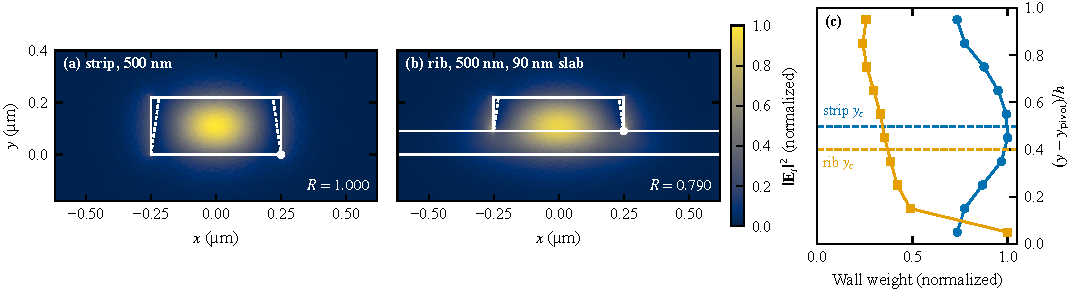
\includegraphics{fig1_sections}
\caption{Why a strip cannot see its sidewall angle. (a)~Oxide-clad strip, \qty{500}{nm}~$\times$~\qty{220}{nm}, and
(b)~rib, \qty{500}{nm} wide on a \qty{90}{nm} slab, both TE at $\lambda=\qty{1.55}{\micro m}$, with the transverse
intensity $|\mathbf{E}_t|^2$, the nominal wall (solid) and a tilted wall (dashed; \qty{8}{\degree}, exaggerated for
visibility) pivoting about the bottom corner (dot). The femwell angle/width ratio $R$ is printed in each panel.
(c)~First-order wall-perturbation weight $W$ along the right wall versus height above the pivot, normalized to its
maximum, with the centroids $y_c$ (dashed). The strip weight is symmetric about mid-height, so a tilt is exactly a width
change ($R=1$); the rib weight sits low on the wall, so $R<1$.}
\label{fig:sections}
\end{figure*}

\begin{figure}[!t]
\centering
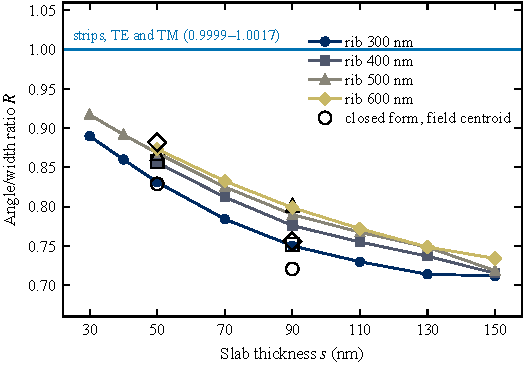
\includegraphics{fig2_ratio}
\caption{Angle/width ratio $R$ of the TE ribs versus slab thickness for four rib widths (femwell derivatives at step
$h$; $\lambda=\qty{1.55}{\micro m}$, $t=\qty{220}{nm}$, oxide-clad). Open symbols: closed form
$R=(y_c-y_\mathrm{pivot})/(h/2)$ from the mode field at the \qty{50}{nm} and \qty{90}{nm} slabs. The line at $R=1$ is
the strip value, set by symmetry. Every rib breaks the strip degeneracy, and thinner slabs break it least.}
\label{fig:ratio}
\end{figure}

\subsection{One rib against unknown etch parameters}

Fig.~\ref{fig:stages} follows a rib on a \qty{70}{nm} slab through the stages (ring and MZI). If the rib shares the
strip angle (stage~B) and only its depth is unknown, one rib width already gives \qty{0.357}{\degree} and two widths
give \qty{0.00365}{\degree}. When the rib has its own angle (stage~C), the single rib leaves the strip angle
unidentifiable, as the count in Section~\ref{sec:structures} predicts, while the two-width set gives
\qty{0.448}{\degree} without priors. Adding $\nsi$, $\nox$ (stage~D) and temperature (stage~E) moves the two-width
bound to \qty{0.481}{\degree} without priors and to \qty{0.452}{\degree} and \qty{0.455}{\degree} with realistic
priors.

\begin{figure}[!t]
\centering
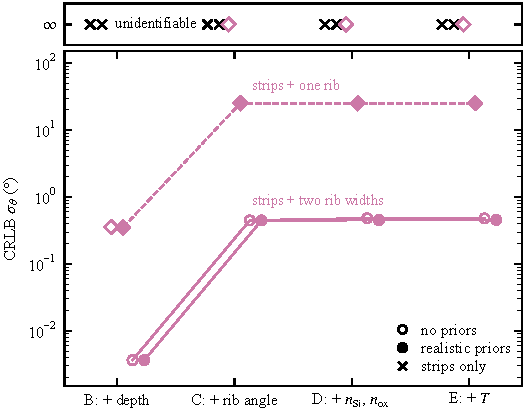
\includegraphics{fig3_stages}
\caption{Strip sidewall-angle CRLB as process unknowns are added (B: etch depth, rib angle tied to the strip angle;
C: separate rib angle; D: silicon and oxide indices; E: temperature), for strips alone (crosses), strips plus one
\qty{500}{nm} rib (diamonds) and strips plus ribs of \qty{500}{nm} and \qty{300}{nm} (circles), all on a \qty{70}{nm}
slab, without priors (open) and with realistic priors (filled), at $\sigma_\lambda=\qty{1}{pm}$, ring and MZI. Cases
with a singular Fisher matrix are drawn in the band marked $\infty$. A second width of the same rib keeps the angle
identifiable once the partial etch has its own angle.}
\label{fig:stages}
\end{figure}

With a single rib whose etch angle is independent of the strip's (stage~C, \qty{70}{nm} slab, \qty{1}{pm}), prior
knowledge improves the bound only partially. Realistic priors give $\sth=\qty{25.18}{\degree}$, knowing the etch depth to
\qty{0.01}{nm} (far beyond what a separate thickness measurement provides) gives \qty{5.03}{\degree}, and tying the rib
and strip angles to within \qty{1}{\degree} gives \qty{1.25}{\degree}. Two widths of the same rib reach
\qty{0.448}{\degree} at the same stage without any of these assumptions. In stage~D with realistic priors, the single
rib gives between \qty{24.4}{\degree} and \qty{45.4}{\degree} depending on the slab, values set by the priors.

\subsection{Multi-width rib sets}
\label{sec:multi}

The two-width set consists of strip TE rings at the five widths plus ribs of \qty{300}{nm} and \qty{500}{nm} on a
\qty{50}{nm} slab. Read by rings alone it gives $\sth=\qty{0.3932}{\degree}$; with an MZI per structure it gives
\qty{0.3891}{\degree} (\qtyrange{0.3891}{0.3997}{\degree} over steps). It is insensitive to derivative errors. On a
fixed mesh the bound (ring and MZI) is \qty{0.394}{\degree}, a \qty{1.3}{\percent} change, and random errors of
$\pm\qty{0.3}{\percent}$ on every \qty{300}{nm}-rib derivative spread it only between \qty{0.364}{\degree} and
\qty{0.420}{\degree} (5th to 95th percentile).

The exhaustive search finds lower bounds with more rib widths and some TM strips. Among ring-only sets, the best set
of eight (TE strips of 400, 550 and \qty{600}{nm}, a TM strip of \qty{400}{nm}, and ribs of 300, 400, 500 and
\qty{600}{nm} on a \qty{90}{nm} slab) gives \qty{0.1895}{\degree}, and the best sets of four to seven give 0.4356,
0.3606, 0.2029 and \qty{0.1941}{\degree}. With an MZI per structure, the best set of eight (TE and TM strips of
\qty{400}{nm} and \qty{600}{nm} and the same four ribs) gives $\sth=\qty{0.139}{\degree}$
(\qtyrange{0.101}{0.147}{\degree} over steps). This set is more sensitive to derivative accuracy than the two-width
set. With fixed-mesh derivatives for the \qty{300}{nm} rib its bound becomes \qty{0.118}{\degree}
(\qty{-15.3}{\percent}), the fixed-mesh and remeshed derivatives differing by at most \qty{0.78}{\percent}, and random
$\pm\qty{0.3}{\percent}$ errors spread it between \qty{0.109}{\degree} and \qty{0.189}{\degree}. We therefore quote
\qtyrange{0.12}{0.14}{\degree} for it, with a derivative-accuracy uncertainty of about \qty{15}{\percent}.

A greedy search that adds one structure at a time reached the exhaustive optimum in 25 of the 32 stage, prior and slab
cases we compared and fell short in 7, with a bound up to a factor of 1.12 larger. At the best-case \qty{0.1}{pm}
precision both ring-and-MZI bounds shrink tenfold, to \qty{0.0408}{\degree} for the two-width set and
\qty{0.0139}{\degree} for the best set. They scale linearly with $\sigma_\lambda$ (\qty{0.196}{\degree} and
\qty{0.775}{\degree} for the two-width set at 0.5 and \qty{2}{pm}).

\subsection{Ring and MZI readout}
\label{sec:mzi}

For the two-width set, adding an MZI per structure lowers the bound from \qty{0.3932}{\degree} (rings only) to
\qty{0.3891}{\degree}. If the MZI phase is three times noisier than our derived value, the bound is
\qty{0.3925}{\degree}; at ten times it is \qty{0.3932}{\degree}, the ring-only value. For the best set of eight the
MZI matters more, \qty{0.1901}{\degree} without it and \qty{0.1390}{\degree} with it, but a threefold noisier MZI
already gives \qty{0.1815}{\degree}. The MZI gain therefore depends on locating a broad fringe as precisely as a narrow
resonance, an assumption we cannot support from the literature, and we base the proposal on rings.

\subsection{Monte Carlo fits reach the bound}

\begin{figure*}[!t]
\centering
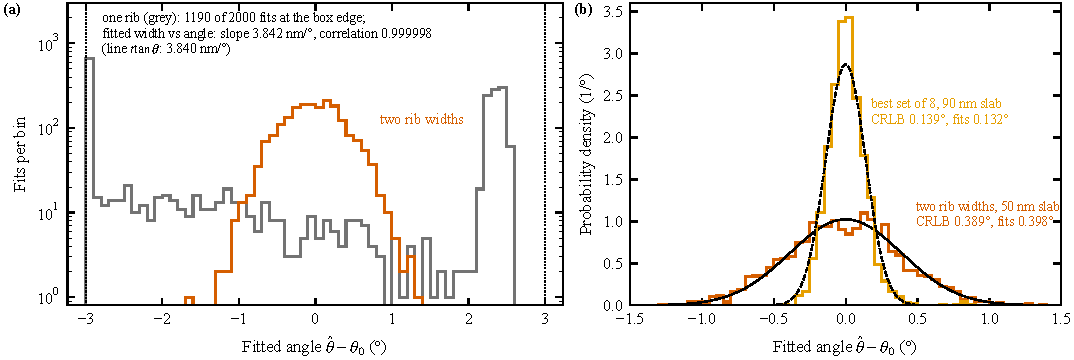
\includegraphics{fig4_montecarlo}
\caption{Monte Carlo fits of 2000 simulated noisy measurement sets per set at $\sigma_\lambda=\qty{1}{pm}$
(stage~D, realistic priors, ring and MZI, bounded nonlinear least squares on the surrogate model). (a)~Histograms of
the fitted strip angle for strip TE rings at five widths plus one \qty{500}{nm} rib (grey) and plus ribs of
\qty{300}{nm} and \qty{500}{nm} (orange), both on a \qty{50}{nm} slab; dotted lines mark the $\pm\qty{3}{\degree}$ fit
box. With one rib the fits spread over the whole box along the width/angle valley. (b)~Fitted-angle histograms for the
two-width set and the best set of eight (\qty{90}{nm} slab) with Gaussians of the CRLB width (lines). With two or more
rib widths the fit scatter matches the bound.}
\label{fig:mc}
\end{figure*}

Fig.~\ref{fig:mc} compares the nonlinear fits with the bound. For the two-width set the fitted angles have a standard
deviation of \qty{0.398}{\degree} (\qtyrange{0.385}{0.410}{\degree}, 95\% bootstrap interval), 1.02 times the CRLB,
with a bias of \qty{-0.015 \pm 0.0089}{\degree}; none of the 2000 fits failed, ended ambiguous or reached the box edge.
For the best set the spread is \qty{0.132}{\degree} (\qtyrange{0.125}{0.140}{\degree}), 0.952 times the CRLB, with a
bias of \qty{0.0075 \pm 0.003}{\degree}; 4 fits ended at the box edge and none failed. The spread is slightly below the
femwell CRLB because the surrogate's own bound at nominal is \qty{0.1249}{\degree}; its \qty{300}{nm}-rib slopes are a
smooth fit through the remeshing scatter. With one rib the fits find the valley predicted by the symmetry argument. The
linearized bound is \qty{29.52}{\degree}, so the $\pm\qty{3}{\degree}$ fit box confines the estimates, and the data do
not: 1190 of the 2000 fits end at the edge of the box, 12 are ambiguous and 20 fail. The fitted widths and angles lie
on a line of slope \qty{3.842}{nm} per degree with a correlation of 0.999998, against
$t\tan(\qty{1}{\degree})=\qty{3.8401}{nm}$ (Fig.~\ref{fig:mc}(a)).

% numbers from results_review/data/surrogate_check.json (HEADLINE_NUMBERS.md section P)
\subsection{Monte Carlo on femwell data}
\label{sec:surrcheck}

The fits above take both the data and the model from the surrogate, so they cannot show what the surrogate's own
errors do to the estimate. For each of the two sets we drew 20 parameter vectors from the CRLB covariance, solved
every structure at each of them with femwell on the r12 mesh (160 solves for the best set, 140 for the two-width set),
and used these mode indices as noiseless data. Each data set received 25 noise realizations at
\qty{1}{pm}, giving 500 fits per set, all made with the surrogate as the model and the settings above.

At these geometries the surrogate follows the strips to within $0.8627\,\sigma_\phi$ in $\neff$, and its $\ngr$ errors
stay below $0.0524\,\sigma_{\ngr}$. The \qty{300}{nm} ribs are again the weak point. On the \qty{50}{nm} slab their
$\neff$ misses femwell by $5.166\,\sigma_\phi$ RMS and by $12.42\,\sigma_\phi$ at worst, and on the \qty{90}{nm} slab
by $1.519\,\sigma_\phi$ and $3.366\,\sigma_\phi$.

The two-width set does not pass these errors on to the angle. Its fitted angles scatter by \qty{0.4034}{\degree}
(\qtyrange{0.3781}{0.4273}{\degree}, 95\% bootstrap interval), 1.037 times the CRLB, with a mean error of
\qty{0.02463 \pm 0.01804}{\degree}, and all 500 fits converge inside the box. The best set of eight does not reach its
bound on femwell data. Its spread is \qty{0.2067}{\degree} (\qtyrange{0.1859}{0.2253}{\degree}), 1.487 times the
CRLB of \qty{0.139}{\degree}, and 14 fits end at the box edge, even though the surrogate errors on its
\qty{300}{nm} rib are the smaller of the two. Its bound rests on small differences between four rib widths, and model
errors of about one noise standard deviation in one of them are enough to widen the estimate. The derivative checks
of Section~\ref{sec:multi} and the variation analysis of Section~\ref{sec:variation} show the same sensitivity. We
take \qty{0.39}{\degree} for the two-width set as the result that holds with an independent forward model, and the
\qty{0.139}{\degree} of the best set as the bound of a model accurate to better than the noise.


\subsection{Slab thickness}

For the ring-only two-width set the bound depends strongly on the slab (Fig.~\ref{fig:slab}). It is lowest at
\qty{50}{nm} (\qty{0.3932}{\degree}), rises slowly toward thinner slabs, to \qty{0.4079}{\degree} at \qty{40}{nm} and
\qty{0.4202}{\degree} at \qty{30}{nm}, and rises quickly toward thicker ones, to \qty{0.6001}{\degree} at \qty{90}{nm} and
\qty{4.094}{\degree} at \qty{150}{nm}. With an MZI the values are within \qty{1}{\percent} of these
(\qty{0.389}{\degree}, \qty{0.403}{\degree}, \qty{0.414}{\degree}, \qty{0.597}{\degree} and \qty{4.089}{\degree}).
Among the slabs simulated the optimum is therefore \qty{50}{nm}. Thinner slabs bring $R$ closer to 1
(Fig.~\ref{fig:ratio}), but we have not separated that effect from the other ways the slab changes the two rib modes.

\begin{figure}[!t]
\centering
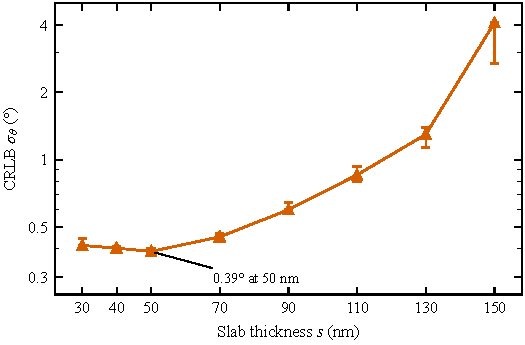
\includegraphics{fig5_slab}
\caption{CRLB of the two-width set (strip TE rings at 400--\qty{600}{nm} plus ribs of \qty{300}{nm} and
\qty{500}{nm}) versus slab thickness, stage~D, realistic priors, $\sigma_\lambda=\qty{1}{pm}$, ring and MZI,
$\lambda=\qty{1.55}{\micro m}$. Bars span the derivative steps $h/2$, $h$, $2h$. The bound is lowest at \qty{50}{nm}
and grows tenfold by \qty{150}{nm}.}
\label{fig:slab}
\end{figure}

\subsection{Measurement-model variants}
\label{sec:noise}

Fig.~\ref{fig:noise} shows how the two headline sets (ring and MZI) respond to departures from the baseline noise
model. A correlation between the $\neff$ and $\ngr$ errors of a ring lowers the bound. At the derived
$\rho=-1/\sqrt2$ the two-width set gives \qty{0.3365}{\degree} and the best set \qty{0.1142}{\degree}, and at
$\rho=0.9$ they give \qty{0.2996}{\degree} and \qty{0.0795}{\degree}. Treating the errors as independent is therefore
conservative.

A wavelength-calibration offset common to all rings matters for the two-width set. Left unknown, it raises the
two-width bound to \qty{1.070}{\degree}; known to \qty{10}{pm}, it gives \qty{0.3892}{\degree}, the baseline. The best
set barely notices the offset (\qty{0.1393}{\degree} unknown). The two-width set therefore needs an absolute
wavelength reference good to about \qty{10}{pm}.

Temperature as a shared unknown changes little. With a prior of \qty{1}{K} the two-width bound is
\qty{0.3917}{\degree}, and with no prior \qty{0.4122}{\degree}; the best set stays at \qty{0.1390}{\degree}. An
independent temperature drift of each structure between its readouts is more damaging. At \qty{10}{mK} per structure the
two-width set gives \qty{0.3935}{\degree} and the best set \qty{0.1877}{\degree}, and at \qty{100}{mK} they give
\qty{0.4599}{\degree} and \qty{0.4993}{\degree}. Larger, multi-structure sets therefore need tighter
thermal control.

\begin{figure}[!t]
\centering
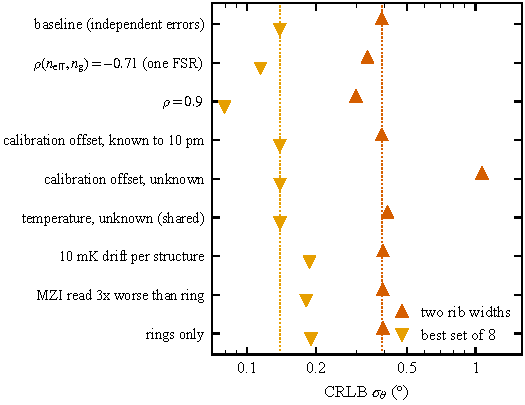
\includegraphics{fig7_noise}
\caption{Strip-angle CRLB of the two-width set (up triangles) and the best set of eight (down triangles) under variants
of the measurement model: stage~D, realistic priors, \qty{1}{pm}, ring and MZI unless the row states otherwise. Dotted
lines mark the baselines. Correlated ring errors lower the bound; an unknown calibration offset harms only the
two-width set; per-structure temperature drift and a noisier MZI harm mainly the best set.}
\label{fig:noise}
\end{figure}

\subsection{Departures from shared process parameters}
\label{sec:variation}

Every bound so far assumes that all structures in a set share one width offset, one thickness and one angle per etch.
A departure common to all structures is absorbed into these parameters. Departures that differ between structures are
not, and the fit converts them into a strip-angle error. For the two-width set the root-mean-square bias gain is
\qty{219.7}{\degree} of strip-angle bias per degree of independent per-structure angle offset, and \qty{57.62}{\degree}
per nanometre of independent width offset; for the best set the gains are \qty{194.1}{\degree} and \qty{74.41}{\degree}.
Per-structure angle offsets with a standard deviation of \qty{0.25}{\degree} thus bias the two-width estimate by
\qty{54.92}{\degree} (standard deviation), and width offsets of \qty{0.5}{nm} bias it by \qty{28.81}{\degree}. An
angle that changes linearly with waveguide width, by \qty{0.25}{\degree} per \qty{100}{nm}, biases the two-width
estimate by \qty{6.869}{\degree} and the best set by \qty{-36.93}{\degree}. Under such departures the shared-parameter
fit returns no useful angle.

If the departures are modeled as unknowns with a Gaussian prior (a random-effects model), the fit stays unbiased and
the bound grows instead (Fig.~\ref{fig:variation}). For the two-width set, per-structure angle departures of
\qty{0.01}{\degree} raise the bound to \qty{0.5502}{\degree}, and \qty{0.1}{\degree} raises it to \qty{2.295}{\degree};
width departures of \qty{0.1}{nm} raise it to \qty{1.139}{\degree}, and thickness departures of \qty{0.1}{nm} to
\qty{2.544}{\degree}. The bound doubles at a per-structure spread of \qty{0.01749}{\degree} in angle,
\qty{0.03938}{nm} in width or \qty{0.01705}{nm} in thickness. The best set is about ten times less tolerant. Its bound doubles at
\qty{0.001739}{\degree} in angle and \qty{0.00365}{nm} in width, and in thickness already below the smallest spread we
evaluated (\qty{0.001}{nm}). The extra structures that make the best set precise are the ones whose small differences the
fit cannot tell apart from the angle.

\begin{figure*}[!t]
\centering
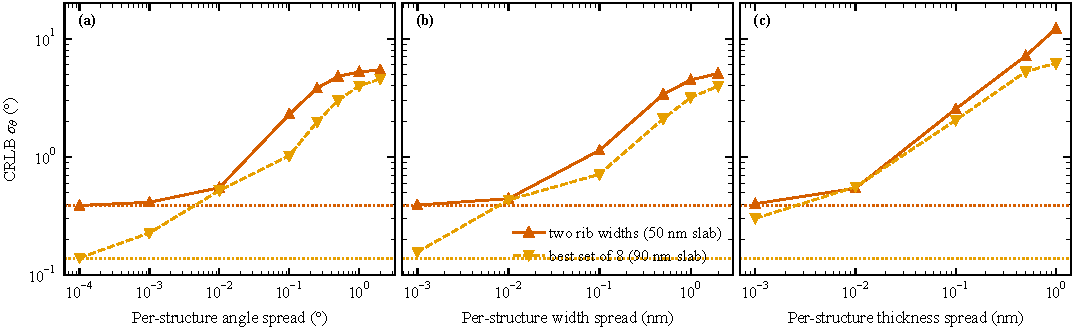
\includegraphics{fig6_variation}
\caption{Strip-angle CRLB when each structure may depart from the shared process parameters (random-effects model),
versus the per-structure spread of (a)~the sidewall angle, (b)~the width and (c)~the thickness, for the two-width set
and the best set of eight (stage~D, realistic priors, \qty{1}{pm}, ring and MZI). Dotted lines: shared-parameter CRLB.
The bound doubles at spreads of a few hundredths of a nanometre or degree for the two-width set, and ten times less for
the best set.}
\label{fig:variation}
\end{figure*}

\subsection{Resonance prediction}
\label{sec:prediction}

When strip rings are fitted with the angle held at its nominal value, a real \qty{1}{\degree} tilt is absorbed as a width
change of \qty{-3.84}{nm}. Using that width to predict a \qty{500}{nm} rib ring on a \qty{90}{nm} slab, whose angle
sensitivity differs ($R<1$), mispredicts its resonance by $\delta\lambda=\lambda\,\delta\neff/\ngr=\qty{-710.8}{pm}$ per
degree of unmodeled tilt.

With the angle in the model, the question becomes how well the extracted parameters predict other devices on the same
chip. We propagate the full parameter covariance of the two-width set to the resonance of a ring, using
$\sigma_{\lambda,\mathrm{pred}}=\lambda\sqrt{\mathbf{g}^{\mathsf T}\mathbf{C}\mathbf{g}}/\ngr$, where $\mathbf{g}$ is the
gradient of the device's $\neff$ and $\mathbf{C}$ is the inverse Fisher matrix. At \qty{1}{pm}, a strip TE ring of
\qty{500}{nm} is predicted to \qty{0.457}{pm} and a rib ring of \qty{500}{nm} on the \qty{50}{nm} slab to
\qty{0.773}{pm}. The angle uncertainty alone would give hundreds of picometres, but it is correlated with the width and
thickness uncertainties, and the combination that sets the resonance is well determined. With an unknown calibration
offset the prediction degrades to \qty{982.2}{pm}, because the two-width set cannot separate the offset from the
process parameters. For the best set the two devices are predicted to \qty{0.559}{pm} and, for the rib on its
\qty{90}{nm} slab, \qty{0.521}{pm}; with the offset unknown the strip ring is predicted to \qty{39.68}{pm}.

\section{Discussion}
\label{sec:discussion}

\subsection{What the numbers mean for a foundry}

Width and thickness monitors made of strips cannot report the sidewall angle of an oxide-clad full etch, however
many they are and in whichever polarization. The cost of that blindness is a misprediction of rib devices of
\qty{710.8}{pm} per degree of tilt. That is comparable to the \qty{841.5}{pm} within-die spread that Zortman \textit{et~al.}\
reported for microdisks, whose across-wafer spread was \qty{8.014}{nm}~\cite{zortman2010}, and well above the
\qty{\pm 32}{pm} accuracy reached by trimming~\cite{jayatilleka2021}. A bound of
\qty{0.39}{\degree} on the angle sounds coarse next to these numbers. What a designer uses, however, is the predicted
resonance of other devices, and within the shared-parameter model the two-width set predicts a strip ring to
\qty{0.457}{pm} and a rib ring to \qty{0.773}{pm} at a \qty{1}{pm} readout (Section~\ref{sec:prediction}). The angle
is uncertain, but the combination of angle, width and thickness that sets each resonance is not. That prediction
needs an absolute wavelength reference to about \qty{10}{pm}; without one it degrades to \qty{982.2}{pm}.

\subsection{When the shared-parameter assumption breaks}

The central limitation is the assumption, shared by every multi-device extraction~\cite{nrc2026}, that all
structures of a set see the same process. Section~\ref{sec:variation} shows that the angle extraction is far more
sensitive to it than a width or thickness extraction. The bound of the two-width set doubles once the structures'
widths differ by \qty{0.03938}{nm} or their angles by \qty{0.01749}{\degree}, and uncorrected offsets of
\qty{0.25}{\degree} produce biases of tens of degrees. For comparison, the best linewidth control reported for a
CMOS line is \qty{0.6}{nm} within a chip~\cite{selvaraja2010}, and the mismatch between identical rings grows with
their separation~\cite{chrostowski2014}, with layout-dependent systematic components~\cite{xing2023}. The closest
measured number is from Xing \textit{et~al.}, who extracted nominally identical waveguides at 44 sites on one die. Their width
had a standard deviation of \qty{1.26}{nm}, and after removing a linear trend across the die the local variation
between nearby devices still reached \qty{3}{nm}, against \qty{0.5}{nm} for the thickness, with an extraction error of
\qty{0.37}{nm} in width~\cite{xing2018}. These
are differences between copies of one design, and the quantity that matters here, the difference between adjacent
waveguides of different widths after the shared offset is removed, has not been reported. If it is of the size Xing
\textit{et~al.}\ measured, the shared-parameter bound is not reachable. A per-structure width spread of
\qty{0.5}{nm} already raises the two-width bound to \qty{3.38}{\degree} (Fig.~\ref{fig:variation}(b)).

A working angle test structure therefore has to meet a consistency requirement that width monitors do not face. Its
members must be close enough, and similar enough in local pattern density, that their departures from one another
stay below a few hundredths of a nanometre, or the design must measure those departures. Two consequences follow for
design. First, the two-width set tolerates about ten times larger departures than the best set of eight, so the
smaller set is the better proposal even though its shared-parameter bound is higher. Second, linewidth depends on local pattern density~\cite{xing2023}, and if the angle does too it can
change systematically with waveguide width; a trend of \qty{0.25}{\degree} per
\qty{100}{nm} biases the two-width estimate by \qty{6.869}{\degree}. Width ranges should therefore be kept narrow, or
the trend added to the model as one more parameter.

\subsection{Relation to physical metrology}

Cross-sections and AFM measure the profile directly at a few sites and remain the reference for calibrating any
optical extraction~\cite{orji2018,yoo2022}. Scatterometry is fast but model-based~\cite{raymond2005}, and its targets
are designed with the same Fisher-information tools we use here~\cite{klein2025,silver2007}. The optical structures
studied here measure the effect of the angle on the guided modes, which is the quantity a circuit depends on, at
every place where rings can be placed. They need a calibrated cross-section model to turn that effect into degrees,
and the co-location requirement above to make the conversion meaningful.

\subsection{Limitations}

The results are simulations, and no device was fabricated or measured. The symmetry argument is first-order and holds
for oxide above and below the core. An air-clad strip is not mirror-symmetric (its angle/width ratio in our solves is
0.9782), and we computed no bound for air-clad sets. The walls are ideal trapezoids tilting about their bottom edge,
without corner rounding or roughness, the material indices are nominal values without dispersion, and $\ngr$ uses a fixed
\qty{5}{nm} wavelength step; none of these choices was varied. Rings are assumed to have known resonance orders and
lengths, so that each resonance gives $\neff$ directly. Only a common calibration offset was tested, and an unknown
length per ring was not. Our $\neff$ noise at \qty{1}{pm} is below the fitting error of measured MZIs
(Section~\ref{sec:theory}), so the measurement model may be optimistic for $\neff$. The bounds scale linearly with
$\sigma_\lambda$ and depend on the noise conversion by tens of
percent. Halving or doubling the rib noise relative to the strips changes the two-width bound by
\qty{-47.9}{\percent} and \qty{97.5}{\percent}, and the ring length used in the conversion changes it by
\qty{-49.4}{\percent} at \qty{50}{\micro m} and \qty{97.8}{\percent} at \qty{200}{\micro m}. The priors matter much
less, at most \qty{0.6}{\percent} for factor-of-two changes. The two-width bound carries a numerical uncertainty of
about \qty{5}{\percent}, the change when the domain is enlarged. The best set of eight is limited by derivative accuracy,
moving by \qty{-15.3}{\percent} between remeshed and fixed-mesh derivatives and by \qty{-27.5}{\percent} at half the
derivative step, and fits of femwell data spread 1.487 times its bound (Section~\ref{sec:surrcheck}). We treat the rib and strip angles as independent because the two etches are separate steps, and
Section~\ref{sec:results} shows how much a link would help. The analysis covers TE ribs only and the
\qty{1.55}{\micro m} band.

\subsection{Next steps}

The decisive experiment is a test chip that carries the two-width set in a compact layout next to conventional width
monitors, measured at controlled temperature against an absolute wavelength reference and compared with
cross-sections of the same dies. Repeating the set at several separations on the chip would measure the local
departures that Section~\ref{sec:variation} identifies as the limit. On the modeling side, per-structure departures
could be absorbed by structures whose members share most of their waveguide, or by the single-ring, many-resonance
approach of~\cite{nrc2026} extended to a rib. TM ribs, air cladding and other platforms such as silicon nitride, where
the cladding and etch profile differ, remain open.

\section{Conclusion}
\label{sec:conclusion}

Four findings summarize this study. To first order, oxide-clad strip waveguides cannot report their sidewall angle, because their mirror
symmetry makes a tilt equivalent to a width change. One rib from a separate etch leaves the angle unidentifiable. Two
widths of the same rib restore it, and simulations indicate a bound of \qty{0.39}{\degree} for five strip rings and two rib rings on a
\qty{50}{nm} slab at a \qty{1}{pm} wavelength precision, reached by nonlinear fits of data from direct mode solutions when the structures share one set of
process parameters. Fabrication consistency is the practical limit. Random offsets at the levels reported for real
processes raise the bound of one copy of the set to several degrees, and joint fits of $N$ copies recover it as
$1/\sqrt{N}$, with tens of copies needed to return within twice the shared-parameter bound. Offsets that follow a design do not average, and
a fabricated test chip must show whether they stay within a few hundredths of a nanometre.


\section*{Acknowledgment}
\todo{acknowledgments: funding, lab, people}

\bibliographystyle{IEEEtran}
\bibliography{refs}

\end{document}
